%! Author = a
%! Date = 1/27/25


\chapter{Arrival}\label{ch:cn_arrival}
Welcome to China!
Hope that you had a nice flight.
You are almost at your destination, so let me guide you through the final steps.

\section[Roaming]{Roaming}\label{sec:cn_arrival_roaming}
\begin{figure}[H]
	\centering
	\begin{minipage}{0.45\textwidth}
		\centering
		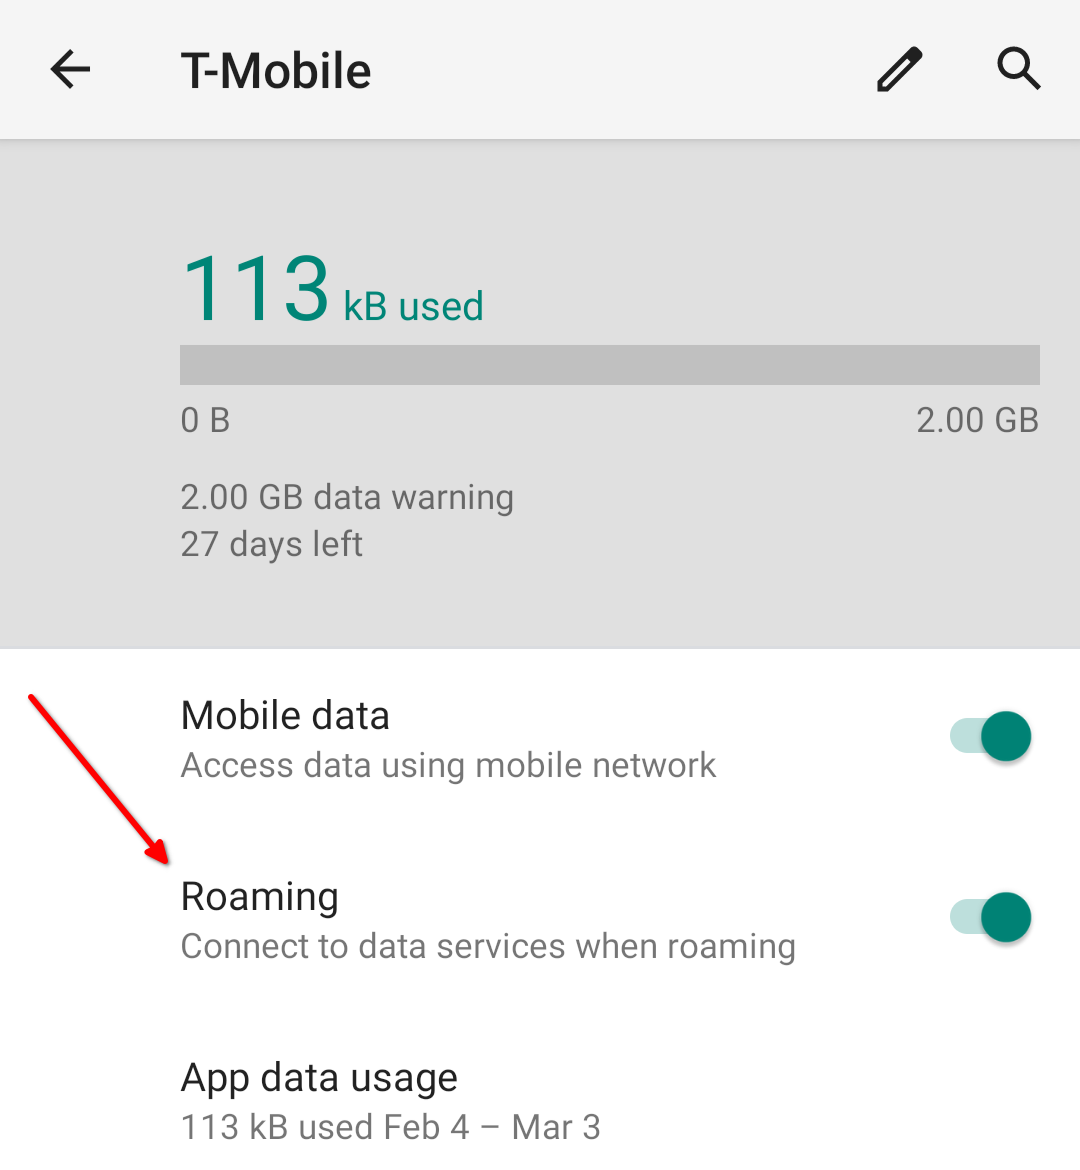
\includegraphics[width=\linewidth]{02_china/images/01_disable_roaming}
		\caption{Roaming option}
	\end{minipage}%
	\hfill
	\begin{minipage}{0.45\textwidth}
		\centering
		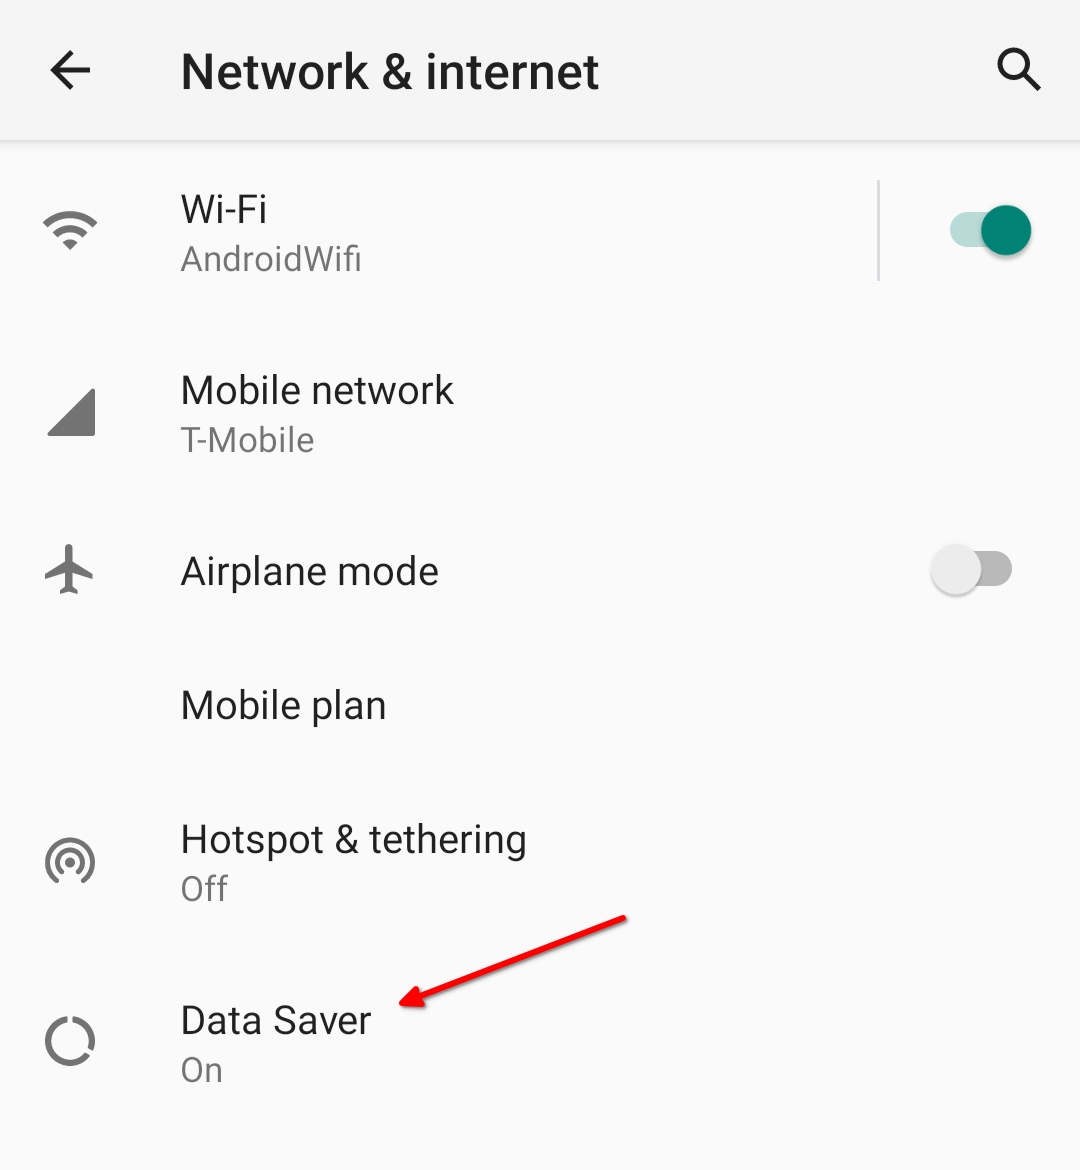
\includegraphics[width=\linewidth]{02_china/images/01_data_saver}
		\caption{Data Saver option}
	\end{minipage}
	\label{fig:cn_disable_roaming}
\end{figure}

Disable the Roaming option in your phone settings.
You should be still able to receive SMS, but your phone won't burn your money.
The prices for the Internet in roaming may be as high as $\textdollar1$ for $\SI{1}{\mega\byte}$.
Please check your carrier pricing.

However, while you are in roaming, you are not subjected to China's Internet restrictions.
So, you will be able to use Telegram, WhatsApp, Google services.
If you are sure that you have enough money on your balance, and you really need to keep access to the Internet, enable the roaming.
You can also enable the Data Saver option, so only the necessary apps have access to the Internet.

\section[Leaving the aircraft]{Leaving the aircraft}\label{sec:cn_leaving_the_aircraft}